\LARGE
\begin{center}
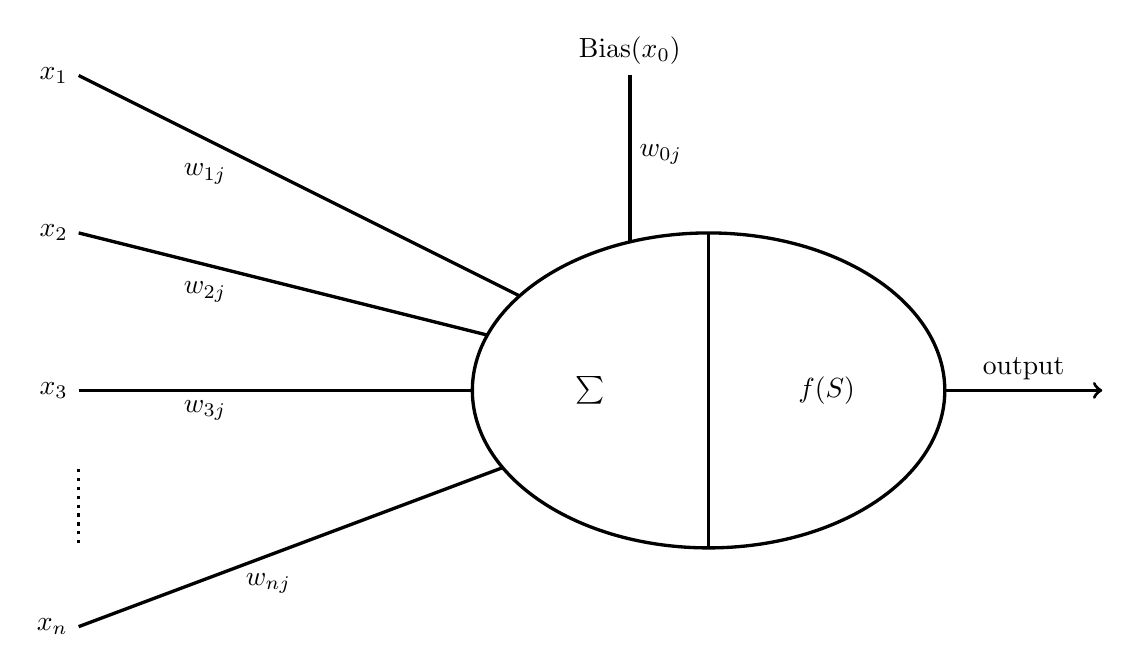
\begin{tikzpicture}

        \draw[very thick] (-1, 4) node[anchor=south]{Bias($x_0$)} -- (-1, 0);
        \draw[very thick] (-8, 4) node[anchor=east]{$x_1$} -- (0, 0);
        \draw[very thick] (-8, 2) node[anchor=east]{$x_2$} -- (0, 0);
        \draw[very thick] (-8, 0) node[anchor=east]{$x_3$} -- (0, 0);
        \draw[very thick, dotted] (-8, -1) -- (-8, -2);
        \draw[very thick] (-8, -3) node[anchor=east]{$x_n$}-- (0, 0);

        \node[anchor=west] at (-1, 3){$w_{0j}$};
        \node[anchor=north east] at (-6, 3){$w_{1j}$};
        \node[anchor=north east] at (-6, 1.5){$w_{2j}$};
        \node[anchor=north east] at (-6, 0){$w_{3j}$};
        \node[anchor=north west] at (-6, -2.2){$w_{nj}$};

        \draw[very thick, fill=white] (0, 0) ellipse (3 and 2);
        \draw[very thick] (0, 2) -- (0, -2);
        
        \node at (-1.5, 0){$\sum$};
        \node at (1.5, 0){$f(S)$};

        \draw[very thick, ->] (3, 0) -- (4, 0) node[anchor=south]{output} -- (5, 0);

\end{tikzpicture}
\end{center}
\normalsize
